\chapter{Saddle point approximation}
\label{cha:sp_approx}

%A semi-classical analysis of ATI which describes the formation of the
%ionization spectrum based on the interference of quantum paths is
%included in Sec.~\ref{sec:spa}. The direct ionization regime is
%considered independently in Sec.~\ref{sec:spa_direct}. The analysis
%presented in this chapter closely follows that
%of~\cite{KopoldOptComm2000}.

%\section{\label{sec:spa} Saddle point approximation}

For laser fields of sufficiently high intensity, the \textsc{ati}
spectrum can be generated by implementing a saddle point
evaluation~\cite{LewensteinSPA_1994} of the multidimensional integral
for the transition amplitude obtained in the previous chapter. This
semi-classical approximation provides a deeper physical insight than
the expansion in Bessel functions from the improved Keldysh
approximation~\cite{Kopold_1997sfa} as it captures the essential
underlying physics. It also establishes a connection between
\textsc{ati} calculations within the framework of the strong-field
approximation and the concept of quantum
paths~\cite{KopoldOptComm2000}, which represent space-time
trajectories of the tunneling electrons. This concept has its origins
in the alternative formulation of quantum mechanics introduced by
Feynman in terms of path integrals~\cite{RevModPhysFeynman}, where the
probability amplitude of a quantum mechanical process can be
represented as a coherent superposition of contributions from all
possible spatio-temporal paths that connect the initial and final
state of the system.

The analysis presented in this chapter establishes the connection
between the quantum mechanical path integral formalism and the
improved Keldysh approximation discussed in Sec.~\ref{kopold_sfa}. The
transition amplitude that describes the ionization of an electron
under an external laser field is evaluated within the two frameworks,
that in which only direct electrons are considered as well as the case
that incorporates rescattering off the parent ion. Our study follows
those in Refs.~\cite{Kopold_1997sfa, KopoldOptComm2000}.

% see pra51 lewenstein

% mention that now that the matrix element for ionization has been
% introduced in the previous chapter, we are going to discuss an
% approximation to obtain the ionization spectrum where the integral
% over time is solved based on the stationary points method

\section{\label{sec:q_paths} Quantum-orbit formalism}
% formalism that derives the equations that describe the quantum paths
% and transition probability within the framework of spa

% describe the physics of the the three-step model where t, t' and k
% are introduced
Several quantum models have been introduced in the literature that
extend the scope of Keldysh approximation for strong laser-atom
interactions~\cite{LewensteinSPA_1994,Lewenstein_1995,Kopold_1997sfa}. These
models, which incorporate rescattering effects of the excited
electrons, have been valuable in unraveling the physical phenomena
behind the \textsc{ati} plateau and its cutoff, an intrinsic feature
of the ionization spectrum. A quasi-classical analysis of this
generalization, based on the saddle point method and the path integral
formalism~\cite{KopoldOptComm2000,Becker_ellipticalSPA,LewScience2001},
has been particularly useful as it elucidates fundamental aspects of
the physics underlying strong-field ionization processes as well as
the formation of their spectra. This approach suggests that one
pictures the processes taking place in laser-atom interactions, such
as \textsc{ati} and high-harmonic generation (\textsc{hhg}), in terms
of electron trajectories in phase space. These quantum trajectories
follow classical Newtonian dynamics, however, must take place in the
complex plane to account for tunneling. Consequently, they present
non-zero imaginary components which determine the probability of the
process. Their physical content is reflected in the electron dynamics
once it has been ionized at time $t'$, the electron may return to its
parent ion at a later time $t$ and rescatter after propagating with
momentum $\mathbf{k}$ in the continuum under the action of the
external field.

In the length gauge, the compact form of the Volkov state can be
expressed as
\begin{eqnarray}
\label{eq:volkov_Lgauge}
\begin{split}
|\psi_{\mathbf{p}}^{(V)}(t)\rangle & = &
|\mathbf{p} - e\mathbf{A}(t)\rangle e^{-i S_{\mathbf{p}}(t)},
\end{split}
\end{eqnarray}
where $|\mathbf{p} - e\mathbf{A}(t)\rangle$ represents a plane-wave
state and
$S_{\mathbf{p}}(t) = 1/2m \int\limits^{t} d\tau [\mathbf{p} -
e\mathbf{A}(\tau)]^{2}$
denotes the action of the system. Consequently, the Volkov
time-evolution operator can be written down in the form of an
expansion in terms of its Volkov states
\begin{eqnarray}
\label{eq:te_volkov}
\begin{split}
U^{(V)}(t,t') & = & \int d^{3}\mathbf{k}
|\psi_{\mathbf{k}}^{(V)}(t) \rangle
\langle \psi_{\mathbf{k}}^{(V)}(t')|.
\end{split}
\end{eqnarray}

Inserting the expansion~(\ref{eq:te_volkov}) into the matrix
element~(\ref{eq:mp_compact}) and given the time dependence of the
ground state wave function,
$|\psi_{0}(t) \rangle = \exp{(iE_{0}t)} | \psi_{0} \rangle$,
one may write~\cite{KopoldOptComm2000}
\begin{eqnarray}
\label{eq:me_action}
\begin{split}
M_{\mathbf{p}} = & \int\limits_{-\infty}\limits^{\infty} dt
\int\limits_{-\infty}\limits^{t} \int d^{3}\mathbf{k}
\ \langle \mathbf{p} - e\mathbf{A}(t) | V | \mathbf{k} - e\mathbf{A}(t) \rangle
\ \langle \mathbf{k} - e\mathbf{A}(t') | V | \psi_{0} \rangle \\
&
\times
\exp \left[i\left(-\frac{1}{2m} \int\limits_{t}\limits^{\infty}
d\tau [\mathbf{p} -e\mathbf{A}(\tau)]^{2} -
\frac{1}{2m} \int\limits_{t'}\limits^{t} d\tau [\mathbf{k} -e\mathbf{A}(\tau)]^{2} +
\int\limits_{-\infty}\limits^{t'} d\tau |E_{0}|
\right)
\right] \\
\sim &
\int\limits_{-\infty}\limits^{\infty} dt
\int\limits_{-\infty}\limits^{t} dt'
\int d^{3}\mathbf{k} \exp \left[ iS_{\mathbf{p}}(t, t', \mathbf{k}) \right]
m_{\mathbf{p}}(t, t', \mathbf{k}).
\end{split}
\end{eqnarray}
As one may notice, the action in the exponent, $S_{\mathbf{p}}(t, t',
\mathbf{k})$, contains three terms which correspond to the action of
the entire system after rescattering, between ionization and
rescattering and before ionization, respectively.

% point out the contrast with feynman's path integral
% p-57 chapter
It is revealing to point out the contrast of the ionization
amplitude~(\ref{eq:me_action}) obtained with the strong field
approximation with its analogous representation in terms of Feynman's
theory of path integral. The time evolution operator of the entire
system has the path integral representation
\begin{eqnarray}
\label{eq:te_path}
\begin{split}
U(\mathbf{r}t, \mathbf{r}'t') & = &
\int\limits_{(\mathbf{r}',t')\to(\mathbf{r},t)}
\mathcal{D}\left[ \mathbf{r}(\tau) \right] e^{i S(t, t')},
\end{split}
\end{eqnarray}
where $S(t, t') = \int\limits_{t'}\limits^{t} d\tau
\mathcal{L}[\mathbf{r}(\tau), \tau]$ is the action calculated along a
specific path by integrating the Lagrangian of the entire system along
that path, and the integral measure denoted by $\mathcal{D}\left[
  \mathbf{r}(\tau) \right]$ establishes a coherent sum over all
possible paths that connect $(\mathbf{r}t)$ and $(\mathbf{r}'t')$,
independently of whether or not the paths might be followed by the
actual system. This sum is, in fact, an infinite-dimensional
functional of integrals, and can be reduced, within the framework of
the strong-field approximation, to a sum over a few quantum orbits. By
implementing the strong-field approximation we have approximated the
exact action of the system at the various stages of the process:
before ionization, in between ionization and rescattering, and after
rescattering, as~(\ref{eq:me_action}) indicates, where the ionization
amplitude is computed through a sum over the exponential of the action
over a five-parameter set of paths, parametrized by the ionization
time $t'$, the rescattering time $t$ and the canonical momentum of the
orbit in between $\mathbf{k}$~\cite{KopoldOptComm2000}.

The five-dimensional set of paths over which the transition
amplitude~(\ref{eq:me_action}) is evaluated can be reduced further by
implementing a saddle point approximation of the
integral~\cite{KopoldOptComm2000}, in which a handful of relevant
paths remains to be considered. Since the quasi-classical actions in
Eq.~(\ref{eq:me_action}) are proportional to $I_{p}$, $U_{p}$, $p^{2}$
and $k^{2}$, which are large under intense laser fields, the factors
$\exp(-i S/\hbar)$ are rapidly oscillating and the integrals in the
transition amplitude can be approximated by the value of the
integrands at the stationary points, saddle points, of the
quasi-classical actions. The condition
\begin{eqnarray}
\label{eq:S_stationary}
\begin{split}
\frac{\partial S}{\partial q_{i}} & = & 0
\end{split}
\end{eqnarray}
where $q_{i}(i =1, \dots, 5)$ runs over the five variables $t$, $t'$
and $\mathbf{k}$, leads to the saddle-point
equations~\cite{Lewenstein_1995,KopoldOptComm2000}
\begin{eqnarray}
\label{eq:saddle_eqs}
\begin{split}
\left( \mathbf{k} - e\mathbf{A}(t') \right)^{2} = &
-2m|E_{0}| \\
\left( \mathbf{k} - e\mathbf{A}(t)\right)^{2} = &
\left( \mathbf{p} - e\mathbf{A}(t) \right)^{2} \\
(t - t') \mathbf{k} = & \int\limits_{t'}\limits^{t}
d\tau e\mathbf{A}(\tau).
\end{split}
\end{eqnarray}
The solutions $(t_{S}(\mathrm{Re}\ t_{S} > \mathrm{Re}\ t'_{S}),
t'_{S}, \mathbf{k}_{S})$, are known as the stationary points of the
quasicassical action of the system, and define the quantum orbits
which are the essential components in building the ionization spectrum
through the saddle-point approximation. From a physical perspective,
Eqs.~(\ref{eq:saddle_eqs}) ensure the energy conservation at the time
of tunneling, elastic scattering of the electron into its final state
when it returns, and that in fact the electron returns to its parent
ion, respectively. Since $|E_{0}| > 0$ in~(\ref{eq:saddle_eqs}), the
condition of energy conservation at the time of ionization cannot be
satisfied for any real time $t'$. As a consequence, the solutions
$(t_{S}, t'_{S}, \mathbf{k}_{S})$ of the saddle-point equations
describe complex orbits which restrains a straightforward
visualization of the trajectories.

%p-56 chapter ATI
The matrix element~(\ref{eq:me_action}) can now be expressed in terms
of the saddle-point solutions as~\cite{KopoldOptComm2000}
\begin{eqnarray}
\label{eq:Mp_final}
\begin{split}
M_{\mathbf{p}} \sim & \sum\limits_{i} \left( \frac{(2\pi i \hbar)^{5}}
{\mathrm{det} (\partial^{2}S / \partial q_{j} \partial q_{k})_{j,k = 1, \dots, 5}}
\right)^{1/2} \times \exp(i S(t_{S_{i}}, t'_{S_{i}}, \mathbf{k}_{S_{i}})),
\end{split}
\end{eqnarray}
where $q_{i}(i = 1,\dots,5)$ runs over the five variables $t_{S},
t_{S}'$ and $\mathbf{k}_{S}$. The sum~(\ref{eq:Mp_final}) involves a
reduced set of trajectories that are sufficient to approximate the
ionization spectrum through their interferences, constructive or
destrutive.


\section{\label{sec:spa_results} Results}
% mention that we explore the quantum trajecotries that are relevant
% to the ATI spectrum

This section presents the results corresponding to a saddle-point
analysis of the probability amplitude to detect \textsc{ati} electrons
that irradiate from a model-helium atom under a strong laser field of
the form~(\ref{eq:lp_field}). In order to obtain comparable results to
the quantum generalization of the strong-field approximation for a
model helium atom, presented in Chapter~\ref{cha:ati}, the laser
intensity and frequency were set to $I = 10^{15}\ \mathrm{W/cm^{2}}$
and $\hbar\omega = 0.0584\ \mathrm{a.u.}$, respectively.

\subsection{\label{sec:spa_direct} Direct trajectories}

The probability amplitude for detecting an \textsc{ati} electron that
propagates with momentum $\mathbf{p}$ in the continuum as a
consequence of the laser irradiation of an atom, originally in its
ground state, is studied in this section. The action that describes
the electron, bound to an atom with a binding energy $E_{0}$, that is
ionized at time $t_{0}$, without further interaction with the parent
ion, has the form
%
\begin{eqnarray}
  \label{eq:action_direct}
  \begin{split}
  S(t_{0}) & = &
-\frac{1}{2m}\int_{t_{0}}^{\infty}{d\tau [\mathbf{p} - e\mathbf{A}(\tau)]^{2}}
- \int_{-\infty}^{t_{0}}{d\tau E_{0}},
\end{split}
\end{eqnarray}
%
where $\mathbf{A}(t)$ represents the vector potential of the laser
field. As the main contribution to the transition
amplitude~(\ref{eq:Mp_final}) is given by the stationary points of the
action which satisfy the condition $dS_{\mathbf{p}} / dt_{0} = 0$, the
integral~(\ref{eq:Mp_final}) is evaluated by implementing a
saddle-point approximation~\cite{spa_1960}. This consists in expanding
the phase of the integrand, $\Phi(t) = (1/\eta) S(t) = (\omega /
U_{p}) S(t)$, in the vicinity of the points where the phase is
stationary. This results in determining the solutions of
%
\begin{eqnarray}
  \label{eq:stationary_points}
  \begin{split}
    \frac{\partial S}{\partial t_{0}} & = &
    \frac{1}{2m} (\mathbf{p} - e\mathbf{A}(t_{0}))^{2} + |E_{0}| = 0.
  \end{split}
\end{eqnarray}
%
Since the stationary points from Eq.~(\ref{eq:stationary_points}) have
a non-zero imaginary component, it is convenient to split the integral
of the action~(\ref{eq:action_direct}) into the complex plane by
implementing the substitution $\omega t_{0} \to \rm{Re}(\omega t_{0})
+ i\rm{Im}(\omega t_{0})$. For a linearly polarized laser field of the
form~(\ref{eq:lp_field}), the location of the saddle points can be
determined analytically and their real and imaginary components
satisfy the conditions
%
\begin{eqnarray}
  \label{eq:ReIm_eqs}
  \begin{split}
    \cos^{2}(\rm{Re}\ \omega t_{0s}) = & \frac{1}{2}
    \left( 1 + \gamma^{2} + \frac{E_{p}}{2U_{p}} \right)
    - \frac{1}{2}\sqrt{\left( \frac{E_{p}}{2U_{p}} \right)^{2}
    + (1 + \gamma^2)^2 + \frac{E_{p}}{U_{p}}(\gamma^2 - \cos 2\phi)}
    \\
    \cosh(\rm{Im}\ \omega t_{0s}) = & - \sqrt{\frac{E_{p}}{2U_{p}}}
    \frac{\cos\phi}{\cos(\rm{Re}\ \omega t_{0s})},
  \end{split}
\end{eqnarray}
%
where $m = -e = 1$ and $\phi$ is the angle between the momentum
$\mathbf{p}$ and the direction of polarization of the laser field,
$\hat{x}$. The electron energy, as it propagates in the continuum, is
indicated by $E_{p} = p^{2}/2m$. As Eqs.~(\ref{eq:ReIm_eqs}) indicate,
a single electron energy $E_{p}$ is associated with four saddle-points
$\omega t_{0s}$, $s = 1, \dots, 4$, which merge into one another by
complex conjugation. These complex roots are illustrated in
Figure~\ref{fig:sp_direct} for electron energies within the range $(0,
\dots, 6U_{p})$. The contours defined by the saddle points in phase
space illustrate the integration paths to follow in order to obtain
the probability amplitude.

% include plot with the saddle-points for direct trajectories
\begin{figure}
  \centering
  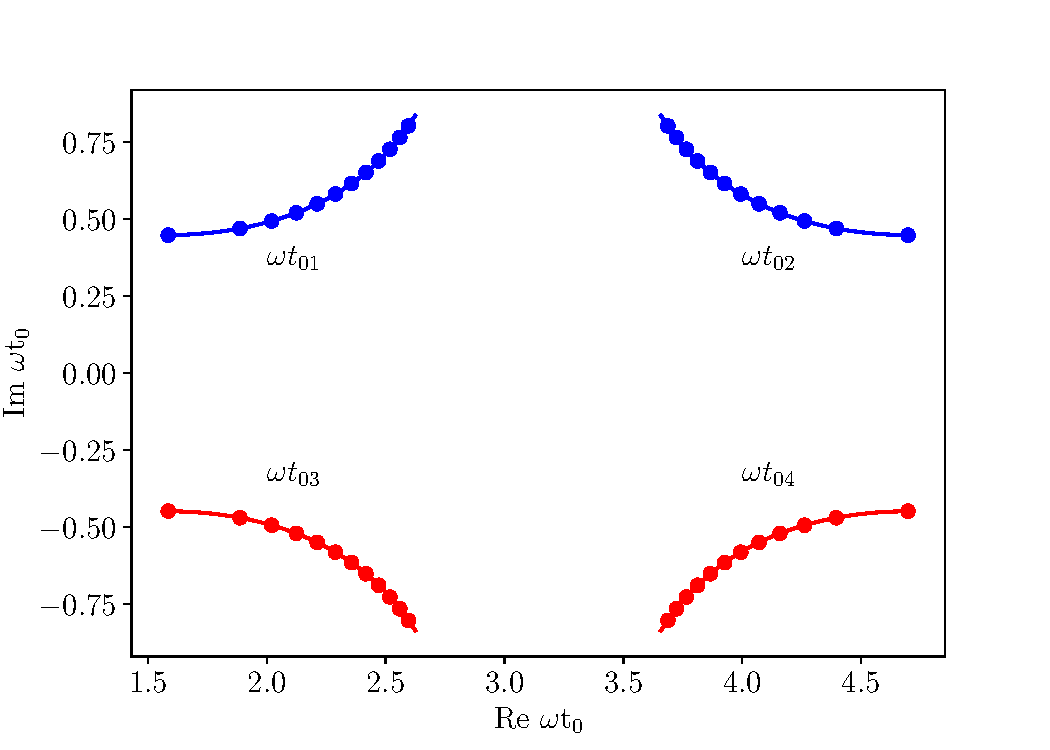
\includegraphics[width = 0.75\textwidth]{figures/ch_ATI_SPA/direct/spDirectElectrons}
  \caption{Saddle points obtained from Eqs.~(\ref{eq:ReIm_eqs})
    associated with direct trajectories of electrons ionized by a
    linearly polarized field with laser intensity of
    $10^{15}\ \rm{W/cm^{2}}$ with $\hbar\omega = 1.58\ \rm{eV}$ for
    electron energies within $E_{p} < 6 U_{p}$.}
  \label{fig:sp_direct}
\end{figure}

A Taylor expansion of the action~(\ref{eq:action_direct}) around the
saddle points allows to approximate the Keldysh-Faisal-Reiss
(\textsc{kfr}) matrix element for direct electrons by a Gaussian
function~\cite{phd_Kopold}
%
\begin{eqnarray}
  \label{eq:KFR_Mp}
  \begin{split}
    M_{\mathbf{p}} & \sim & \int\limits_{0}\limits^{T} dt\ e^{i \eta \Phi(t)},
  \end{split}
\end{eqnarray}
%
where the phase $\Phi(t) = S_{\mathbf{p}}(t)\omega / U_{p}$, and the
period of the laser field is indicated by $T$. The integration path to
follow is defined by a contour of saddle points whose locations, given
by Eq.~(\ref{eq:ReIm_eqs}), are known analitically for a linearly
polarized laser field.

% explain how to choose the relevant contours and the figure in phase space
% then explain eq.B25 from Kopold

In order to visualize the regions in phase-space where the action $S$
is stationary and, consequently, construct an integration path of
stationary phase through the saddle-points, it is convenient to carry
out the substitution $t \to t_{r} + it_{i}$ in
Eq.~(\ref{eq:action_direct}). For a monochromatic laser
field~(\ref{eq:lp_field}), and assuming that the electron path is
parallel to the electric field of the laser, $\phi = 0$, the real and
imaginary components of the phase take the form~\cite{phd_Kopold}
%
\begin{eqnarray}
  \label{eq:phase_im}
  \begin{split}
    \mathrm{Im}(i\Phi(t)) & = & \omega t_{r} ( 1 + \frac{E_{p}}{U_{p}}
    + 2\gamma^{2} ) +
    \frac{1}{2} \sin 2\omega t_{r} \cosh 2\omega t_{i}
    + 2\sqrt{\frac{2E_{p}}{U_{p}}} \sin\omega t_{r} \cosh\omega t_{i}
  \end{split}
\end{eqnarray}
%
\begin{eqnarray}
  \label{eq:phase_re}
  \begin{split}
    -\mathrm{Re}(i\Phi(t)) & = & \omega t_{i} (
    1 + \frac{E_{p}}{U_{p}} + 2\gamma^{2} )
    + \frac{1}{2} \cos 2\omega t_{r} \sinh 2\omega t_{i}
    + 2\sqrt{\frac{2E_{p}}{U_{p}}} \cos\omega t_{r} \sinh\omega t_{i}.
  \end{split}
\end{eqnarray}
%
At a given electron energy, the permited integration contours follow
from $\mathrm{Im}\ i \Phi(t) = \mathrm{Im}\ i \Phi(t_{si})$, and
Eq.~(\ref{eq:phase_im}) allows to write them explicitly as a function
of $t_{i}(t_{r})$. Figure~\ref{fig:sp_contours} shows contours for
constant imaginary part of the exponent in Eq.~(\ref{eq:KFR_Mp}), as
well as the set of saddle points corresponding to an electron energy
of $2.27 U_{p}$. The blue curve corresponds to contours with
$\mathrm{Im}\ i \Phi(t) = \mathrm{Im}\ i \Phi(t_{s_{1},s_{3}})$, while
contours with $\mathrm{Im}\ i \Phi(t) = \mathrm{Im}\ i
\Phi(t_{s_{2},s_{4}})$ are indicated by a red curve. The purple scale
represents the real values of the exponent $i\Phi(t)$, in which dark
regions indicate small values of $\mathrm{Re}\ i\Phi(t)$, while bright
regions indicate large values of $\mathrm{Re}\ i\Phi(t)$. This
indicates that, for every single electron energy $E_{p}$, only one
possible integration path is relevant in order to evaluate the
transmission amplitude $M_{\mathbf{p}}$. The one starting at $t = 0$
to $+i\infty$, $C_{a}$, then along $C_{1}$ across the saddle point
$t_{01}$ up to $\omega t = \pi + i\infty$ where the integrand
vanishes, from there along $C_{2}$ across the second saddle point,
$t_{02}$, to $\omega t = 2\pi + i\infty$, and finally along $C_{b}$ to
$\omega t = 2\pi$. The integrands along $C_{a}$ and $C_{b}$ are
identical and the integrals add up to zero due to the reversed
integration orders. Along contours $C_{1}$ and $C_{2}$ the integrand
is approximated by a Gaussian, which results in~\cite{phd_Kopold}
% explain how to generate the spectrum having obtained the phase
\begin{eqnarray}
  \label{eq:Mp_spa_direct}
  \begin{split}
    M_{\mathbf{p}} & \sim & \sum\limits_{i = 1,2}
    \sqrt{\frac{2\pi\hbar}{-i S''_{\mathbf{p}}(t_{s_{i}})}}
    \exp iS_{\mathbf{p}}(t_{s_{i}}).
  \end{split}
\end{eqnarray}
%
Equation~(\ref{eq:Mp_spa_direct}) approximates the \textsc{ati}
spectrum for an electron that, after being ionized at some time
$t_{0}$ under a strong laser field, propagates within the influence of
the field with no further interaction with the binding potential.

% include contour plots for constant values of Im(\Phi) and
% integration path
\begin{figure}
  \centering
  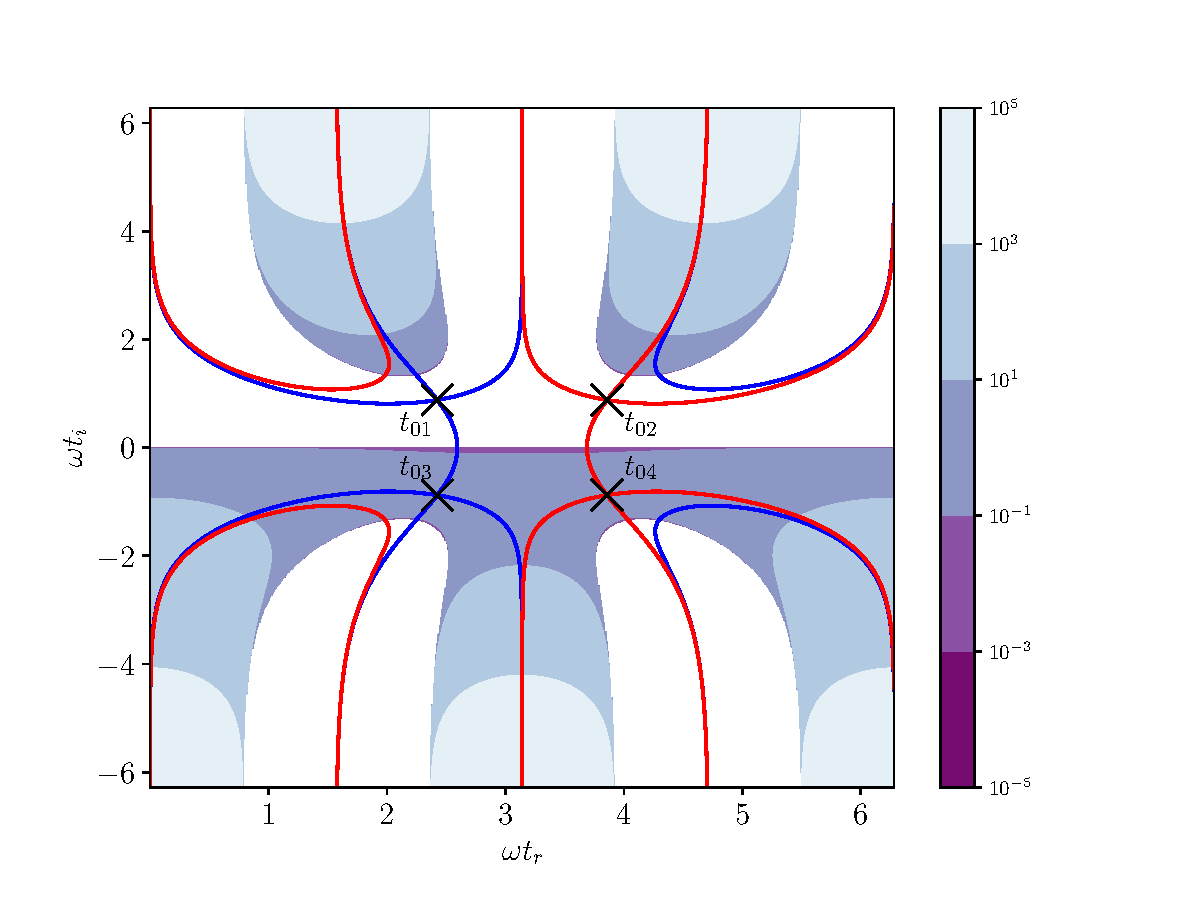
\includegraphics[width = 0.75\textwidth]{figures/ch_ATI_SPA/direct/phase_contour12}
  \caption{Phase contours of constant $\mathrm{Im}\ i\Phi(t)$ for the
    saddle points $t_{01}(t_{03})$ (blue lines) and $t_{02}(t_{04})$
    (red lines) corresponding to an electron energy of $2.27 U_{p}$
    projected on the complex plane. The regions in a purple scale
    represent contours of constant $\mathrm{Re}\ i\Phi(t)$.}
  \label{fig:sp_contours}
\end{figure}

The ionization spectrum of direct electrons for a model helium atom is
calculated by means of the saddle-point approximation, as
Figure~\ref{fig:sp_direct} displays in dash-dotted
lines. Additionally, the \textsc{ati} spectrum corresponding to the
standard Keldysh amplitude is indicated with black dots. For a given
electron energy, $E_{p}$, the probability
amplitude~(\ref{eq:Mp_spa_direct}) was evaluated along the integration
trajectory that contains the saddle-points with positive imaginary
parts, $t_{01}$ and $t_{02}$ indicated in Figure~\ref{fig:sp_direct},
in order to obtain a converging result when evaluating the exponential
term in $M_{\mathbf{p}}$. The complex path of these saddle points is
indicated as blue dots in Fig.~\ref{fig:sp_direct} as the electron
energy increases from $0$ to $4 U_{p}$. The saddle-point approximation
mirrors the fully quantum calculation in terms of an expansion in
Bessel functions. Similarly to what the Keldysh \textsc{sfa} results
point out, the saddle-point approximation generates an \textsc{ati}
spectrum that vanishes at approximately $2.5 U_{p}$ as the electron
escapes the effects of the binding potential without further
interaction with the parent ion.

\begin{figure}
  \centering
  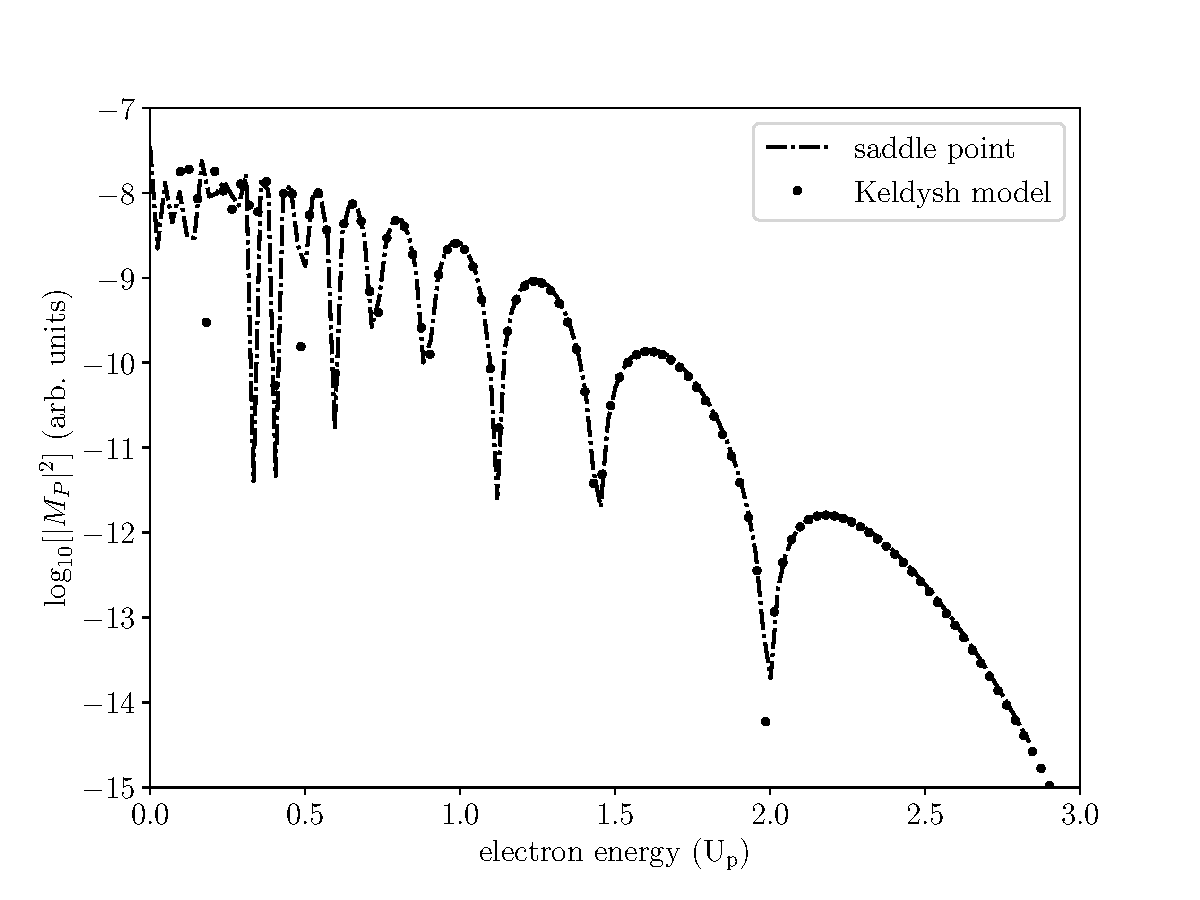
\includegraphics[width = 0.75\textwidth]{figures/ch_ATI_SPA/direct/SPvsKeldysh}
  \caption{Calculated ATI spectrum using Keldysh formalism (black
    dots) and the saddle-point approximation (dash-dot line) in terms
    of trajectories $1$ and $2$, for a laser intensity of
    $10^{15}\ \rm{W/cm^{2}}$, $\hbar\omega = 1.58\ \rm{eV}$, and a
    binding energy of $E_{0} = -0.9\ \rm{a.u.}$ for a zero-range He
    model. With $\gamma = 0.654$ and $\eta = 17.9$.}
  \label{fig:sp_direct}
\end{figure}


\subsection{\label{sec:spa_resc} Trajectories with rescattering}

% fundamental features of rescattering, how is this approached
The introduction of rescattering effects into the study of
\textsc{ati} expands the possible physical interpretations to the
ionization spectrum, in particular, it provides a comprehensible
description to the origin of the \textsc{ati}
plateau~\cite{Paulus_1994plateau,BeckerRescattering_2018}. It is the
purpose of this section to revisit a saddle-point approximation of the
rescattering picture in which the quantum orbits of the ionized
electron play an esential role in the formation of the \textsc{ati}
spectrum~\cite{KopoldOptComm2000}.

% equations to determine the physical magnitudes (t, t', k) that
% define the complex trajectories, i.e., saddle points
In the recollision picture, an electron transitions from the ground
state into the continuum at time $t'_{S}$, ionization time, from that
time on the effects of the laser field in the electron dynamics are
dominant and the Coulomb potential of the parent ion is neglected as
the electron propagates in the continuum with momentum $\mathbf{k}$,
however, the model allows further interaction with the binding
potential and the electron is considered to return to within the
vicinity of the ion at time $t_{S}$, rescattering time, at which the
electron acquires its final asymptotic momentum $\mathbf{p}$. The
relevant quantum trajectories, defined by $(t'_{S}, t_{S},
\mathbf{k}_{S})$, are given by the saddle-point
equations~(\ref{eq:saddle_eqs}) which have their origin in the
condition that the action of the system remains stationary along those
points. For the linearly-polarized field~(\ref{eq:lp_field}), after
some algebraic work on the saddle-point equations, one can solve for
the rescattering time and ionization time as the numerical solutions
of~\cite{KopoldOptComm2000}
%
\begin{eqnarray}
  \label{eq:return_t}
  \begin{split}
    [\omega t_{S} \mp \arccos(2\cos\omega t_{S} + \delta \mp i\gamma)]
    (2\cos\omega t_{S} + \delta) \\
    \pm \sqrt{1 - (2\cos\omega t_{S} + \delta \mp i\gamma)^{2}} 
    - \sin\omega t_{S} = 0
  \end{split}
\end{eqnarray}
%
and
%
\begin{eqnarray}
  \label{eq:release_t}
  \begin{split}
    \omega t'_{S} = \mp \arccos(2\cos\omega t_{S} + \delta \mp i\gamma),
  \end{split}
\end{eqnarray}  
%
respectively, where the quantity $\delta$ is defined as $\delta =
\sqrt{p^{2} / (4mU_{p})}$. Therefore, the complex paths are generated
for every possible set of $(t'_{i}, t_{i}, \mathbf{k}_{i})$. As
Eq.~(\ref{eq:return_t}) indicates for the rescattering time, there are
two possible solutions in each optical cycle $T = 2\pi$ due to the
combination of signs and infinite solutions due to the multivaluedness
of the $\arccos$ function. Considering the periodicity of the laser
field, we can focus our attention to the interval $0 <
\mathrm{Re}\ t_{S} < T$ for the rescattering times. Subsequently,
Eq.~(\ref{eq:release_t}) produces two solutions for the ionization
time within the interval $-T/2 < \mathrm{Re}\ t'_{S} < 0$, two from
the interval $-T < \mathrm{Re}\ t'_{S} < -T/2$, and so
forth. Typically, the travel time $\mathrm{Re}(t_{S} - t'_{S})$
associated to a quantum trajectory indicates the relevance of its
contribution to the \textsc{ati} spectrum, the ones with shorter
travel time being qualitatively more important.

% add algebra on the action for trajectories with rescattering and
% break down into real and imaginary components (based on the electron
% paths being complex to account for tunneling ionization), which is
% later shown in Fig. 5.5
In the rescattering picture, it is illustrating to take into account
the complex nature of the electron dynamics in order to visualize how
the action of the system, $S(t_{i},t'_{i},\mathbf{k})$, evolves as the
electron energy increases. To this end, one can write the explicit
analytic expression for the action in the event that the canonical
momentum $\mathbf{k}$ and the final momentum $\mathbf{p}$ are parallel
to the linearly polarized laser field~(\ref{eq:lp_field}), which reads
%
\begin{eqnarray}
  \label{eq:action_analytic}
S_{\bf{p}}(t, t', \bf{k}) & = &
-\frac{1}{2} \int_{t}^{\infty} d\tau\left[ p^{2}
- 2eA_{0}p\cos(\omega\tau) + (eA_{0})^{2}\cos(\omega\tau)^{2} \right]\nonumber\\
&& -\frac{1}{2} \int_{t'}^{t} d\tau\left[k^{2}
- 2eA_{0}k\cos(\omega\tau) + (eA_{0})^{2}\cos(\omega\tau)^{2} \right]\nonumber\\
&& + \int_{-\infty}^{t'} d\tau|E_{0}|.
\end{eqnarray}
%
In the vicinity of the saddle points $(t_{i},t'_{i},\mathbf{k})$,
where the action is stationary, the integration limits that cause the
integrand to diverge to $\pm\infty$ can be neglected. Some algebraic
simplifications on the analytic expression for the action allow us to
express the phase, $\Phi = (1/\eta)S$, in the probability
amplitude~(\ref{eq:Mp_final}) as
%
\begin{eqnarray}
  \label{eq:phase_final}
\Phi(t, t', \bf{k}) & = &
\left(\frac{E_{P}}{U_{P}} - \frac{k^{2}}{2U_{P}}\right) \omega t
+ \frac{2e}{\sqrt{U_{P}}} \left( k - \sqrt{2E_{P}}\right) \sin(\omega t) \nonumber\\
&&
+ \left( \frac{k^{2}}{2U_{P}} + e^{2}+2\gamma^{2} \right)\omega t'
- \frac{2e}{\sqrt{U_{P}}} k\sin(\omega t') \nonumber\\
&&
+ \frac{e^2}{2}\sin(2\omega t'),
\end{eqnarray}
%
where $E_{P}$ indicates the electron energy.

%The phase is defined as Φ = (1/η)S = (ω/UP )S, where UP is the
%ponderomotive energy of the electron. Multiplying the action (12) by
%the 1/η factor and making use of the definitions of the ponderomotive
%energy and the Keldysh parameter one arrives at the expression


The complex orbits for the ionization time, rescattering time and
complex momentum, given by the saddle-point solutions of
Eqs.~(\ref{eq:return_t}) and~(\ref{eq:release_t}), are shown in
Figure~\ref{fig:complex_paths} for trajectories $i = (1,\dots,6)$ as a
function of the electron kinetic energy $E_{p}$. A subset of the
energy values is indicated in multiples of $U_{p}$ along the paths. In
the process of obtaining the saddle points corresponding to
trajectories with increasing travel times, the substitution $\omega t
\to \omega t + 2\pi k$, with $k = 0,1,\dots$, was implemented in
Eqs.~(\ref{eq:return_t}) and~(\ref{eq:release_t}). The behaviour of
these complex trajectories is markedly different depending on the
location of the classical cutoff. Every pair of trajectories shows
that the quantum orbits approach each other closely near the
cutoff. For energies above the cutoff, the orbits in every pair
diverge away from one another and the ones with negative imaginary
parts stop contributing to the \textsc{ati} spectrum and are dropped
from the sum~(\ref{eq:Mp_final}), as they lead to a diverging solution
for probability amplitude. This cutoff marks a turning point of the
complex paths. As it can be noticed, both the rescattering times and
quantum momentum have very small imaginary parts before the cutoff,
while their imaginary components become noticeable as the electron
energies increase beyond the cutoff. In contrast, the imaginary parts
of the ionization times are significant, indicating the origin of the
electrons through tunneling ionization. For energies above the cutoff,
the real components of the complex paths remain approximately constant
with increasing energy. As a result, a marked drop appears after the
cutoff in the spectrum associated with a given pair of trajectories.

% plot of saddle points
\begin{figure}
\begin{subfigure}[b]{0.33\linewidth}
  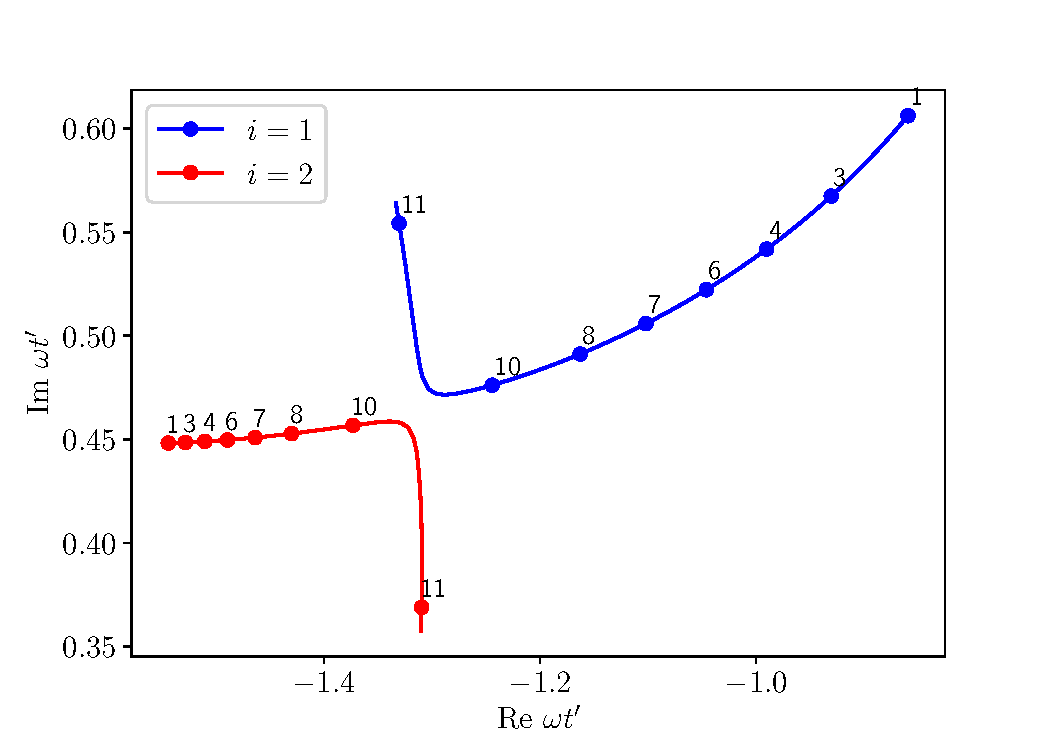
\includegraphics[width=\textwidth]{figures/ch_ATI_SPA/rescattering/start12.pdf}
\end{subfigure}
\begin{subfigure}[b]{0.33\linewidth}
  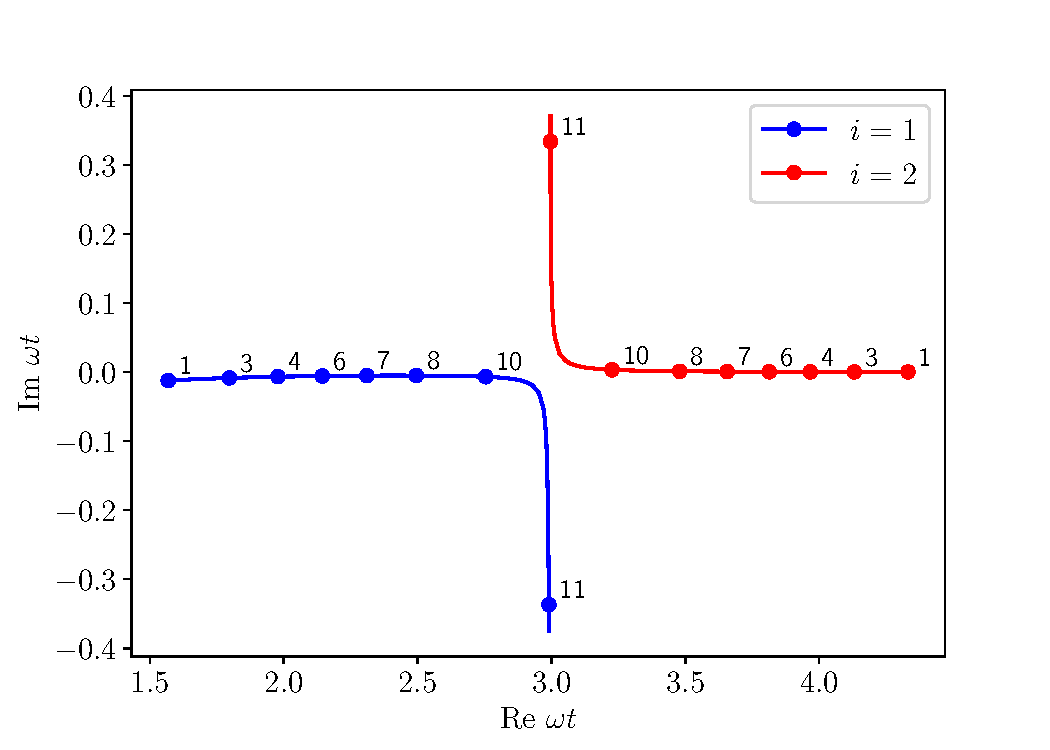
\includegraphics[width=\textwidth]{figures/ch_ATI_SPA/rescattering/return12.pdf}
\end{subfigure}
\begin{subfigure}[b]{0.33\linewidth}
  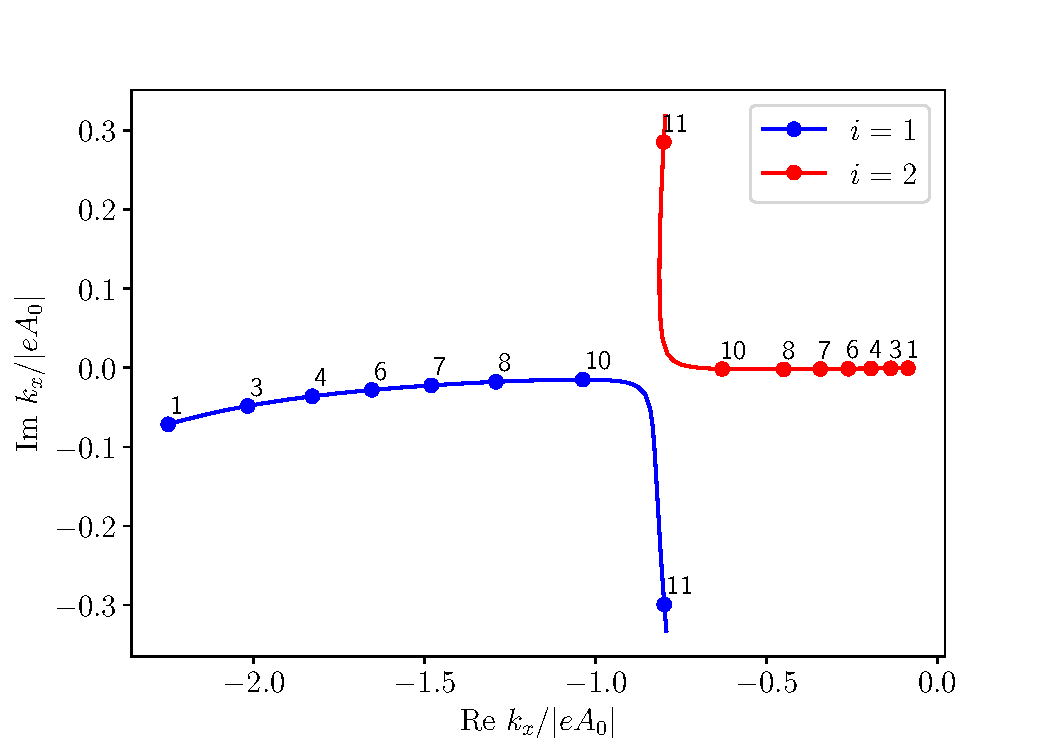
\includegraphics[width=\textwidth]{figures/ch_ATI_SPA/rescattering/momentum12.pdf}
\end{subfigure}
\begin{subfigure}[b]{0.33\linewidth}
  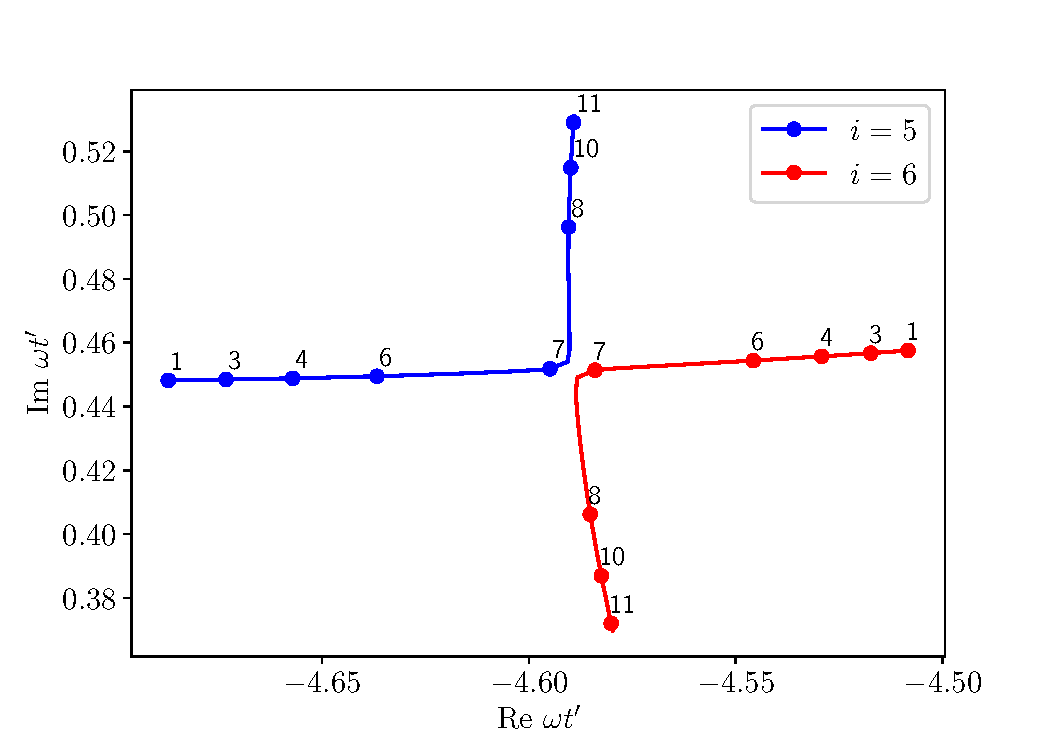
\includegraphics[width=\textwidth]{figures/ch_ATI_SPA/rescattering/start34.pdf}
\end{subfigure}
\begin{subfigure}[b]{0.33\linewidth}
  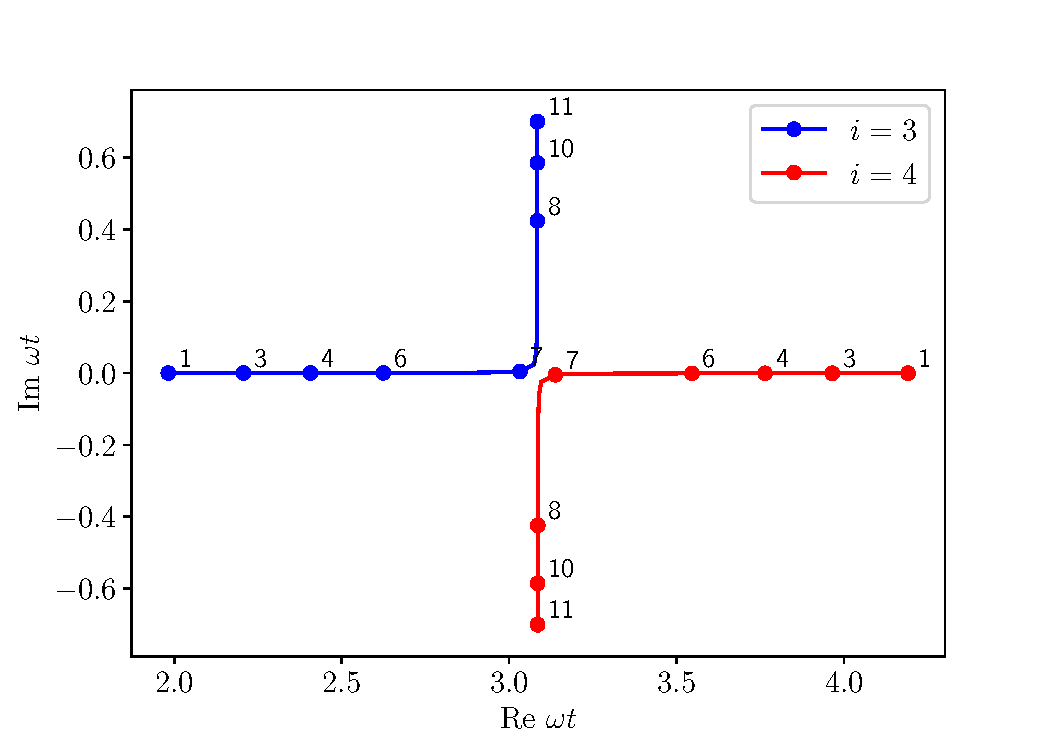
\includegraphics[width=\textwidth]{figures/ch_ATI_SPA/rescattering/return34.pdf}
\end{subfigure}
\begin{subfigure}[b]{0.33\linewidth}
  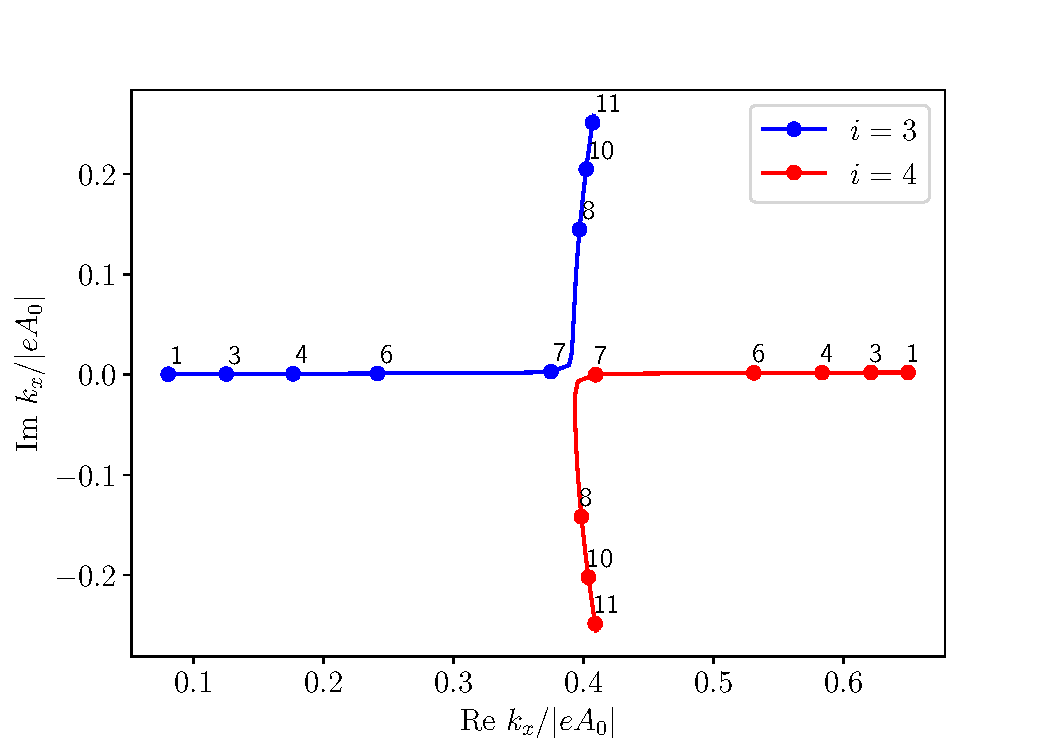
\includegraphics[width=\textwidth]{figures/ch_ATI_SPA/rescattering/momentum34.pdf}
\end{subfigure}
\begin{subfigure}[b]{0.33\linewidth}
  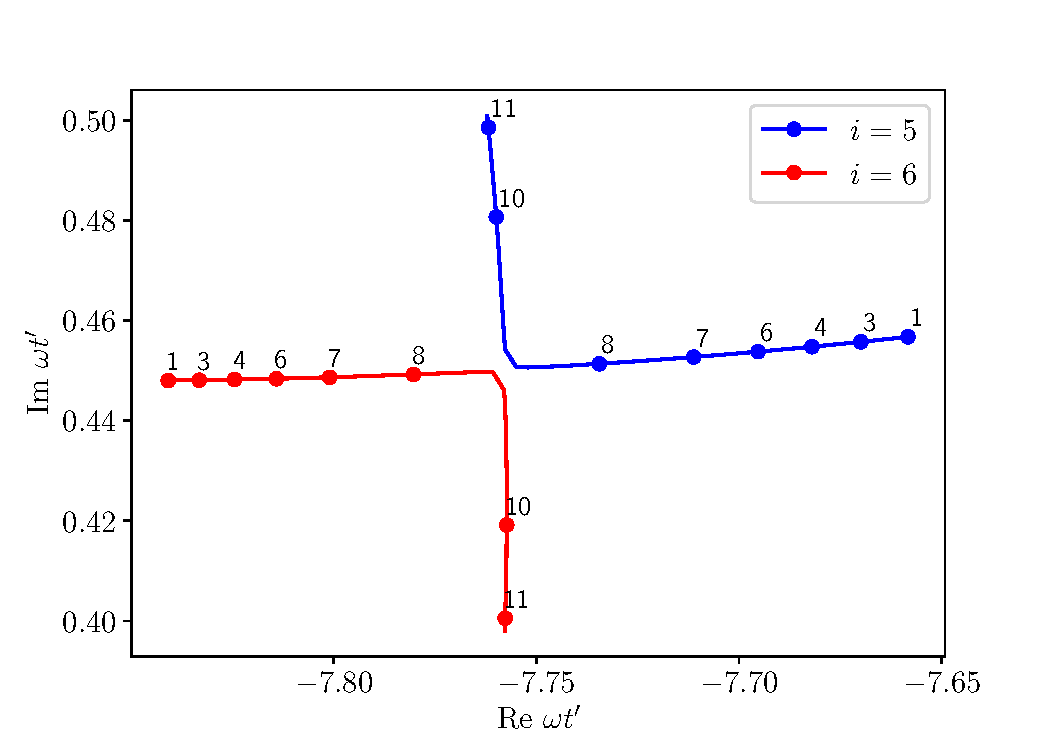
\includegraphics[width=\textwidth]{figures/ch_ATI_SPA/rescattering/start56.pdf}
\end{subfigure}
\begin{subfigure}[b]{0.33\linewidth}
  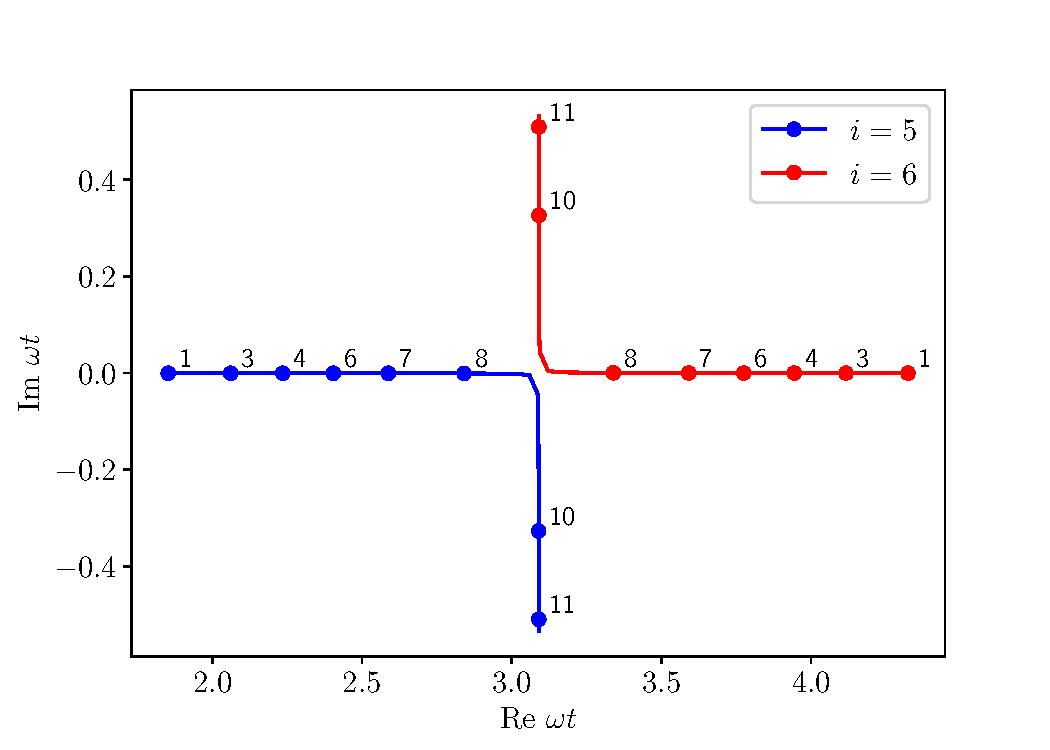
\includegraphics[width=\textwidth]{figures/ch_ATI_SPA/rescattering/return56.pdf}
\end{subfigure}
\begin{subfigure}[b]{0.33\linewidth}
  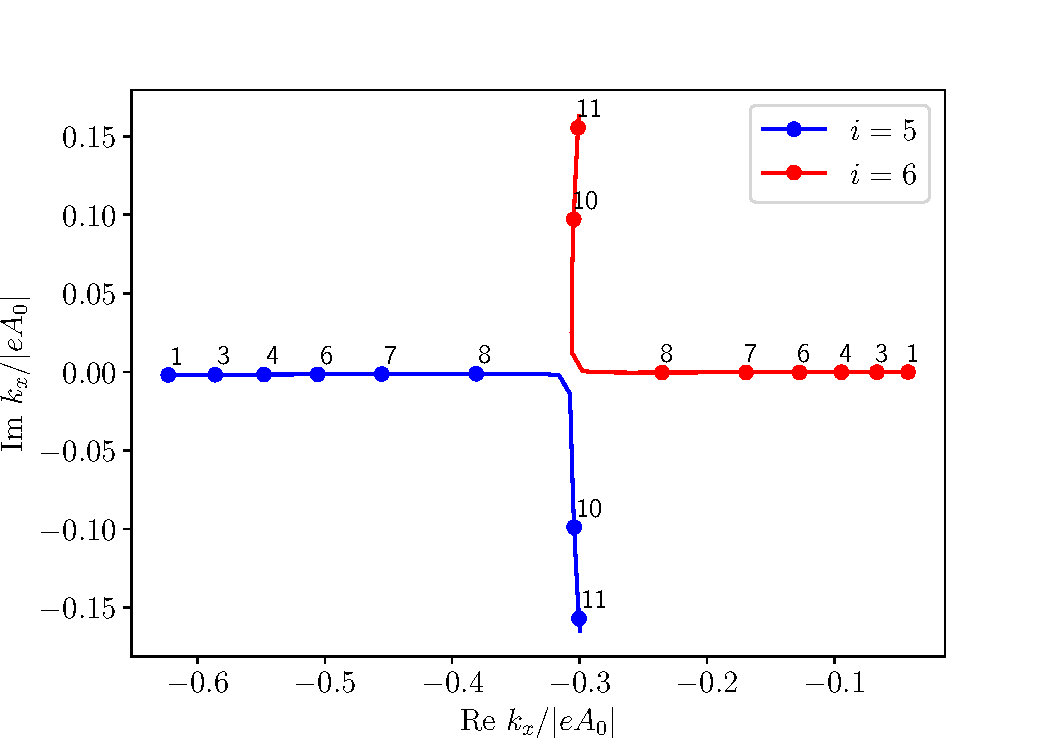
\includegraphics[width=\textwidth]{figures/ch_ATI_SPA/rescattering/momentum56.pdf}
\end{subfigure}
\caption{Saddle points for the orbits $(s = 1,\dots,6)$ in the complex
  plane as a function of the electron energy $E_{p}$ specified along
  the lines in multiples of $U_{p}$. A laser field of
  $10^{15}\ \mathrm{W/cm^{2}}$ and $\hbar\omega = 1.58\ \mathrm{eV}$
  and a binding energy of $E_{0} = -0.9\ \mathrm{a.u.}$ were used in
  the calculations. In this figure, $\omega t'$ represents the
  ionization time, $\omega t$ stands for rescattering time, and
  $k_{x}$ is the $x-$component of the canonical momentum
  $\mathbf{k}$. The underlying Keldysh parameter was set to $\gamma =
  0.464$.}
  \label{fig:complex_paths}
\end{figure}

% write expression of the action that is plotted in the complex plane
The actions $S(t_{i},t'_{i},\mathbf{k}_{i})/\eta$, with $\eta = 35.8$,
corresponding to the electron trajectories with the shortests travel
times $(i = 1, 2)$ are shown in Figure~\ref{fig:phase_ReIm} for
increasing electron energy $E_{p}$. A subset of energy values is
specified along the curves up to the cutoff energy, whereupon a
crossing takes place between the paths. In addition, the complex
coordinates of the action extracted from~\cite{phd_Kopold} are
included for the electron energies specified, $\times$, along with
errorbars that reflect a comparison with the analytical expression for
the action~(\ref{eq:action_analytic}). For energies below the cutoff
the most noticeable changes occur in the real components, while the
imaginary parts of the individual trajectories change little as they
approach each other along the plateau. In contrast to the saddle
points behaviour (Figure~\ref{fig:complex_paths}), where in a given
pair of trajectories $(i, j)$ they diverge rapidly from one another
towards the cutoff, the complex contributions of the action become
more similar as the electron energy increases and eventually are
interchanged at the cutoff, at which point one of the trajectories
ceases to contribute to the \textsc{ati} spectrum.
% MENTION THIS IN THE DESCRIPTION OF THE ATI SPECTRUM FIGURE
% Towards the cutoff, however, the trajectories and their
% contributions become more and more similar. Because of this, the
% last constructive interference at the cutoff is always most
% pronounced. Finally, the weights are interchanged and only one of
% the two trajectories may continue to be taken into account

% plot of action in phase-space
\begin{figure}
  \centering 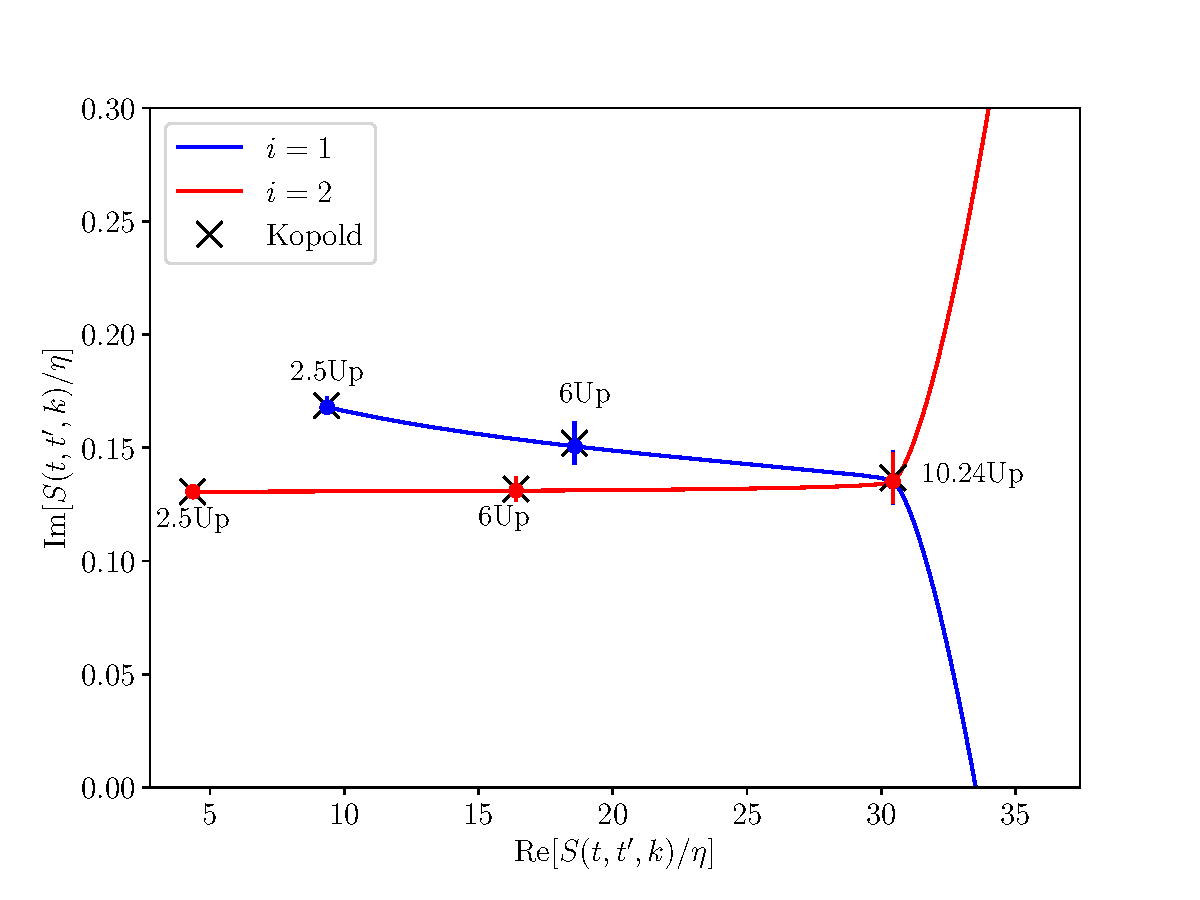
\includegraphics[width =
    0.75\textwidth]{figures/ch_ATI_SPA/rescattering/phase_ComplexReIm.pdf}
  \caption{Representation of the action in the complex plane for the
    two shortest trajectories $(1, 2)$ shown in blue and red
    respectively. In addition, the complex coordinates for the action
    extracted from~\cite{phd_Kopold} are shown as $\times$ for the
    specified energy values.}
  \label{fig:phase_ReIm}
\end{figure}

% mention errorbars in the plot of the action in the complex plane for
% paths 1 and 2

The computation of the \textsc{ati} spectrum can now be carried out
once the solutions of the saddle-point equations are determined. To
this end, the appropriate subset of electron trajectories is inserted
into the matrix element~(\ref{eq:Mp_final}).



% plot of formation of the spectrum as the number of trajectories
% increases






%%% Local Variables:
%%% mode: latex
%%% TeX-master: "thesis"
%%% End:
